\newpage
\section{Color image processing \buch{p.394}}
\subsection{Color fundamentals \buch{p.395}}
\begin{itemize}
	\item Humans can perceive thousands of colors but only about 20-30 shades of gray
	\item Color is often a great feature of object detection and extraction
	\item White light can be split into a spectrum of colors
	\item The human visual system (HVS) is quite complex, but basically, the cones are responsible for the color vision
	\begin{itemize}
		\item There are about 7 million cones which can be put into three categories
		\begin{itemize}
			\item $65\% $ are sensitive to red
			\item $33\% $ are sensitive to green
			\item $2\% $ are sensitive to blue
		\end{itemize}
		\item while their numbers vary widely, their sensitivity is quite similar
		\begin{itemize}
			\item Therefore, the blue cones are the most sensitive
			\item But the spatial resolution of red is much higher than that of blue
		\end{itemize}
	\end{itemize}
	\item Red, Green and Blue are called additive primary colors
	\item Magenta, Yellow and Cyan are called subtractive primary colors
	\item Humans often describe color using
	\begin{description}
		\item[Brightness:] Chromatic notation of intensity
		\item[Hue:] The dominant color
		\item[Saturation:] How much white light is mixed in with the pure color
	\end{description}
	\item The very useful HIS (Hue, Saturation, Intensity) color space is based on the color perception of humans	
\end{itemize}

The amount of red(X), green (Y) and blue (Z) needed to form a given color are called the tristimulus values.
A color can then be specified using its trichromatic coefficients x,y and z, which are normalized so that they sum to 1.
For any wavelength of light in the visible spectrum, these values can be read from tables that are the results from extensive experimentation.

\[
	x = \frac{X}{X+Y+Z} \qquad
	y = \frac{Y}{X+Y+Z} \qquad
	z = \frac{Z}{X+Y+Z}
\]



\subsection{Color models \buch{p.401}}
A color model is also called a color space or a color system. It allows colors to be represented in a well defined way, and depending on the task at hand, one model might be better suited than another.

\subsubsection{RGB model \buch{p.402}}
Based on the three primary colors of the HVS and the most used model as most color camera systems and monitors have these three channels.


\subsubsection{CMY and CMYK model \buch{p.406}}
These are models well suited for the primary colors of pigments, such as used in printing. The K stands for black, which, in theory can be mixed by summing up all subtractive primary colors, but for printing, the result tends to be a bit muddy, hence black is its own color.

\subsubsection{The HSI Color Model \buch{p.407}}
The HSI Color Model is well suited for image procesing algorithms.\\
\begin{minipage}{0.6\textwidth}
\begin{itemize}
	\item \textbf{H} - hue: information about color, determined by an angle from some reference point $\rightarrow$ usually an angle of $0^\circ$ at the red axis.
	\item \textbf{S} - saturation: length from the origin to the abritrary color point
	\item \textbf{I} - intensity: given by the position of the plane on the vertical intensity axis.
\end{itemize}
\end{minipage}
\hspace{0.05\textwidth}
\begin{minipage}{0.35\textwidth}
	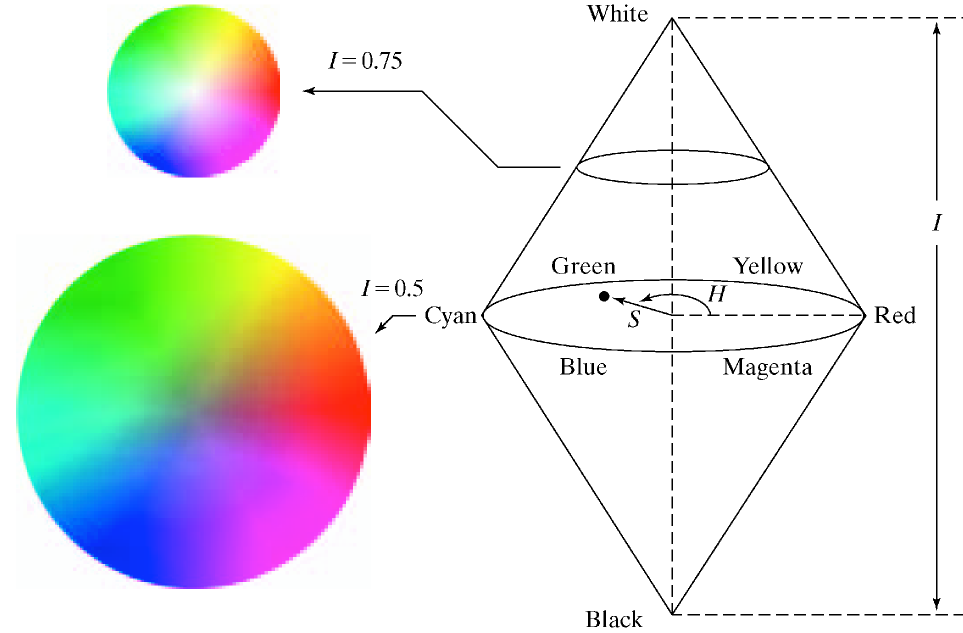
\includegraphics[width = \textwidth]{./images/HSI_ColorSpace}
\end{minipage}

\subsubsection{Converting RGB $\Leftrightarrow$ HSI \buch{p.410}}


\subsection{Pseudo color image processing \buch{p.414}}
\subsubsection{Intensity Slicing \buch{p.415}}
\subsubsection{Intensity to color transformation \buch{p.418}}


\subsection{Color transformations \buch{p.426}}
\subsubsection{Color complements \buch{p.430}}
\subsubsection{Color slicing \buch{p.431}}
\subsubsection{Histrogram processing {p.438}}

\subsection{Smoothing and sharpening \buch{p.439}}
\begin{tabular}{l|l|l}
	& 
	\textbf{RGB} & 
	\textbf{HSI} \\
	
	\textbf{Smoothing \buch{p.439}}&
	Eq. 6.6-2 &
	only I (average)\\
	
	\textbf{Sharpening \buch{p.442}}&
	Eq. 6.6-3 &
	only I (laplace)\\
\end{tabular}

\subsection{Image segmentation based on color \buch{p.443}}
HSI is not perfect for image segmentation $\rightarrow$ RGB method yields better results! $\Rightarrow$ p.445
\subsubsection{Bounding boxes \buch{p.446}}
Simplest method of implementing image segmentation in RGB space 

\subsection{Color edge detection \buch{p.447}}
Two possibilities to detect edges in RGB-color space:
\begin{enumerate}
	\item Use Sobel operators on each color to form the gradient of each RGB component and add them together at each coordinate (x,y)
	\item Vector method described on p.449
\end{enumerate}

\subsection{Noise in color images \buch{p.451}}
Some of the gray scale methods are allowed for full color images.

Other schemes cannot be that easily extended to color images, such as the order statistic filters.